\section{Introduction}
\label{sec:introduction}

\begin{figure}[t]
\centering
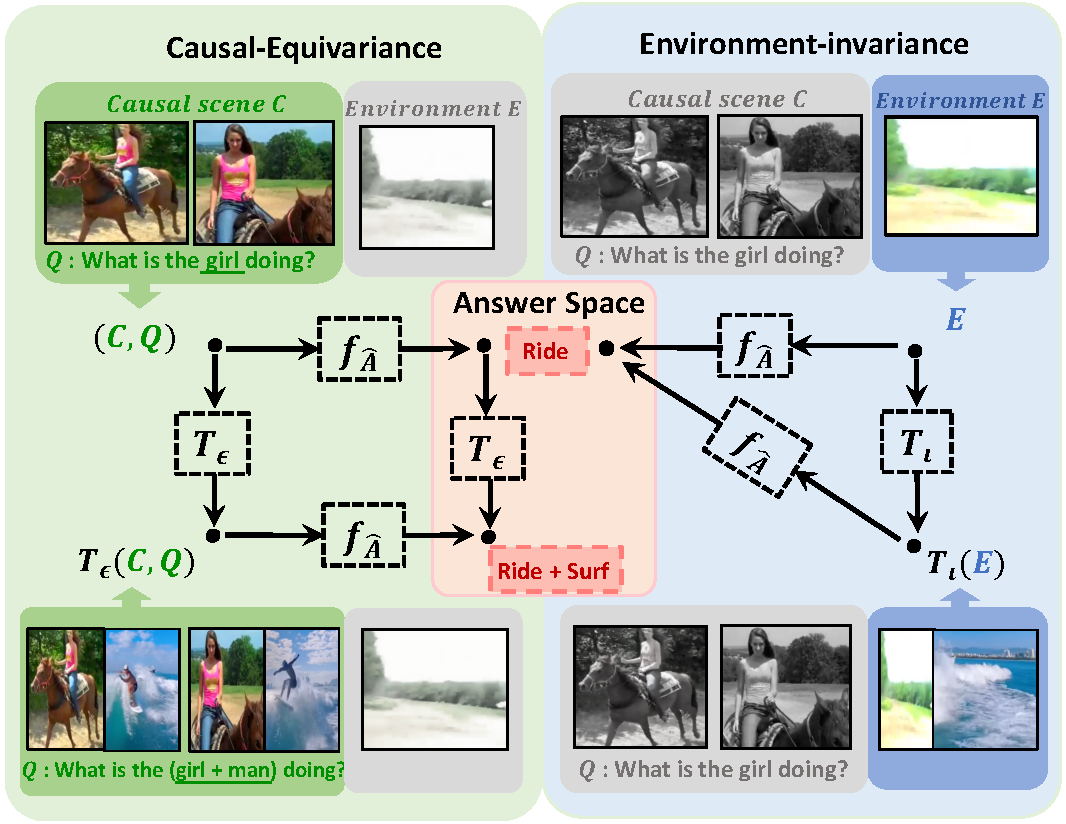
\includegraphics[scale=0.47]{fig/f1.pdf}
\vspace{-15pt}
\caption{
Illustration of equivariant and invariant grounding.
The causal-equivariant principle (left) asks that the semantic change $T_{\epsilon}$ applied to the causal scene $C$ and question $Q$ should be faithfully reflected in the answer change.
In contrast, the environment-invariant principle (right) outputs the same answer, regardless of changes $T_{\iota}$ on the environment scene $E$.
Here, $f_{\hat{A}}$ maps input to answer space.
}
\vspace{-15pt}
\label{fig:overview}
\end{figure}

% 1.videoQA overview-----------------------------------------
Video Question Answering (VideoQA) \cite{zhong2022video} is a keystone in interactive AI, such as vision-language navigation and communication systems.
It aims to answer the natural language question based on the video content.
Striving for the architecture novelty, many studies have been conducted on modeling VideoQA's multi-modal nature, such as fostering the vision-language alignment \cite{jiang2020reasoning,park2021bridge} and revisiting the visual input structure \cite{le2021hierarchical,dang2021hierarchical}.
However, existing VideoQA models usually operate as black boxes, which fail to exhibit the working mechanism behind the predictions and hardly exhibit ``What knowledge should the model use to answer the question about the video?''.
As a result, the black-box nature causes concern for the model's reliability, especially in applications to safety and security.



% 2.problem of interpretable-------------------------------
The concern on the black-box nature calls for  \lyc{better transparency} of VideoQA models.
Here we focus on visual-explainability \cite{CSS,DBLP:conf/ijcai/RossHD17}, aiming to reveal ``Which part of the video should the model look at to answer the question?''.
It requires us to find a subset of visual scenes --- rationale --- \lyc{that support the answering as evidence in way of human interpretation} \cite{DBLP:conf/ijcai/RossHD17}.
Taking Figure \ref{fig:overview} as an example, when answering the question ``What is the girl doing?'', the rationale should focus on the ``girl-riding on-horse'' scene in the first two clips.
Towards this end, existing studies \cite{gao2018motionappearance,DBLP:conf/iccv/Liu0WL21,DBLP:conf/mm/WangG0W21} dwell mainly on the paradigm of \textbf{post-hoc explainability} \cite{LIME,DBLP:conf/iccv/SelvarajuCDVPB17}, which distributes the predictive answer of the target model to the input visual features via an additional explainer method.
They visualize the attention weights or gradient-like signals toward the visual features, and then identify a salient pattern as the rationale.
However, post-hoc explainability has several major limitations:
(1) It fails to make the target model intrinsically interpretable \cite{DBLP:conf/cvpr/YangZQ021,wang2021causal,DBLP:journals/natmi/Rudin19},  only approximating the decision-making process of the model.
As a result, the identified rationale cannot faithfully reveal how the model leverages the multi-modal information.
(2) Such visual inspections are fragile against input perturbations, since some artifacts can be easily captured as explanations instead of genuine knowledge from the data \cite{DBLP:conf/ijcai/LaugelLMRD19,slack2020fooling,heo2019fooling,ghorbani2019interpretation}.




% 3.partition the video to get interpretation ------------
The limitations of post-hoc explainability inspire us to explore the paradigm of \textbf{intrinsic interpretability} \cite{ghorbani2019interpretation,DBLP:journals/natmi/Rudin19}, which embeds a rationalization module into the model to make the decision-making process transparent.
Surprisingly, the intrinsic interpretability of VideoQA models is until-now lacking.
To fill the void, we draw on \textbf{causal theory} \cite{pearl2016causal,pearl2009causal} to formulate the interpretability task as disclosing ``Which part of the video is critical/causal to answering the question?''.
Concretely, we aim to identify the causal component of input video on-the-fly, which holds the question-response information and filters out the question-irrelevant cues.
Following this essence, one straightforward realization is to ground the input video into two segments:
(1) \textbf{causal scene}, which retains the question-critical visual content and sufficiently approaches the answer, thus naturally serving as the rationale;
and (2) \textbf{environment scene}, which holds the question-irrelevant visual content and can be seen as the rationale's complement.



% 4.euiqvariant and invariant -------------------------------
% 要突出的是grounding,title中是Equivariant and invariant grounding,所以要让这些关键词尽早的出现。
% 这个例子融入到下面的Causal-Equivariance和Environmental-Invariance中去。
%
However, discovering causal scene without the supervision of ground-truth rationale is challenging.
With a causal look at the reasoning process (\cf Section \ref{sec:causal-view}), we argue that the crux of intrinsic interpretability is to amplify the connection between the causal scene and the answer, while blocking the non-causal effect of the environment scene.
Following this line, we propose two principles to guide the grounding of the rationale:
\begin{itemize}[leftmargin=*]
    \item \textbf{Causal-Equivariance.}
    By ``equivariance'', we mean that answering should be sensitive to the semantic changes on the causal scene and question (termed E-intervention), \eg any change on the causal scene and question should be faithfully reflected on the predicted answer. For example, in Figure \ref{fig:overview}, the ``girl-riding on-horse'' and ``man-surfing in-ocean'' scenes are the oracle rationales of ``What is the girl doing?'' and ``What is the man doing?'', respectively. The intervention \cite{li2021interventional} applied on the input (\ie mixing the ``girl-riding on-horse'' and ``man-surfing in-ocean'' scene, and combining two questions as ``What is the girl doing? What is the man doing?'') should set off an equivariant change in the answer (\ie changing from ``Ride'' to ``Ride+Surf'').
    
    
    
    \item \textbf{Environment-Invariance.}
    By ``invariance'', we mean that answering should be insensitive to the changes in the environment scene (termed I-intervention), conditioning on the causal scene and question.
    Considering Figure \ref{fig:overview} again, the intervention applied to the environment (\ie mixing the ``meadow'' and ``ocean'' scenes) implies no impact towards answering ``What is the girl doing?'', reflecting a homogeneity in the answer space.
\end{itemize}


%5.overall idea ------------------------------------------------------------------
% Aspiring to capture grounding rationale, we formalize a model-agnostic learning framework, Equivariant and Invariant Grounding for Interpretable VideoQA (EIV), 
% %
% by asking the question ``what and how transformation should the model be equivariant or invariant to?'' 
% %
% Different from the previous effort that design supervised proxy task for geometric transformation \cite{DBLP:conf/iccv/ChengSM21}, 
% % we adopted philosophy of causal intervention and design a saliency-aware temporal mix method for the video input, and impose 
% we answer the ``what'' question by adopting the philosophy of causality \cite{pearl2009causal} and configure transformation as causal intervention operation that imposes scene-aware mixup \cite{DBLP:conf/iclr/ZhangCDL18} on the multi-modal input.
% %
% As for the question of how, we present a unified view of equivariant and invariant principles via the lens of temporal self-supervised learning, where the contrastive counterparts are bred through a disruption on the causal scene, environment scene as well as vision-language alignment.

% where the contrastive counterparts are bred through a disruption on the causal and environment scene, respectively.

% implemetation ----------------------------------------------
% 这一段的写作逻辑应该是如何实现equivariant、invariant principles的;可以不用follow IGV的写法;

% 可以这么组织:
% 一句话介绍三个modules;
% 然后如何用这三个modules来实现两个principle的:首先用grouidng indicator去roughly partition videos into two parts:causal and environmental scenes;然后基于这两部分引入causal-equivariance:利用interventer对于causal scenes做interventions,期望answer部分产生相对应的变化;利用interventer对于environmental scenes做interventions,期待这部分不会对于answering产生影响。

To impose these two principles for intrinsic interpretability, we propose a new framework, \underline{E}quivariant and \underline{I}nvariant \underline{G}rounding for Interpretable \underline{V}ideoQA (\textbf{EIGV}).
EIGV equips the VideoQA backbone model with three additional modules:
a grounding indicator, an intervener, and a disruptor.
First, the grounding indicator learns to attend the causal scene based on the input question, while leaving the rest as the environment.
% However, this grounding only roughly estimates the oracle partition of causal and environment scenes.
Then, the intervener parameterizes the proposed principles to guide the grounding.
Specifically, towards the causal-equivariance principle, it conducts the E-intervention on the causal scene and question --- that is, mix them with the counterparts from another video-question pair --- and encourages the predictive answer to be anticipated accordingly.
Towards the environment-invariance principle, when leaving the causal scene and question untouched, it applies the I-intervention on the environment --- that is, mix it with the environmental stratification of a memory bank --- and enforces the predictive answer to be invariant.
Moreover, we build an unified sight of two principles via the lens of contrastive learning.
Concretely, on top of each intervened video-question pair, the disruptor constructs the positive views by disrupting the environment scene randomly, while creating the negative views by substituting the causal scene with random scenes.
Training with these two principles allows the backbone model to distinguish the causal scene from the environmental cues, and hinge on the critical visual-linguistic alignment. 


Briefly put, our contributions are: 
\begin{itemize}[leftmargin=*]
    \item We propose EIGV, a model-agnostic VideoQA framework that distills the causal visual-linguistic alignment to generate answers in a self-interpretable manner.
    
    \item We investigate the soundness of grounding rationale by posing the equivariant-invariant principle on visual grounding.
    
    \item We justify the superiority of EIGV on three popular benchmark datasets (\ie MSVD-QA \cite{DBLP:conf/mm/XuZX0Z0Z17}, MSRVTT-QA \cite{DBLP:conf/mm/XuZX0Z0Z17},  NExT-QA \cite{DBLP:conf/cvpr/XiaoSYC21}) with extensive experiments, where our design outmatches the state-of-the-art models. Moreover, our EIGV is a model-agnostic framework that can be applied to different VideoQA models. 
\end{itemize}













